\documentclass[10pt]{article}
\usepackage[margin=2.2cm]{geometry}
\usepackage[T1]{fontenc}
\usepackage{lmodern}
\usepackage{microtype}
\usepackage{booktabs}
\usepackage{amssymb,amsmath}
\usepackage{listings}
\usepackage{xcolor}
\usepackage{tikz}
\usetikzlibrary{positioning}
\usepackage{hyperref}
\lstset{basicstyle=\ttfamily\small, breaklines=true, columns=fullflexible, keepspaces=true}
\newcommand{\code}[1]{\texttt{#1}}
\title{\vspace{-1.2em}Formalizing Hardware in \textsf{lean-surfaces}\\[2pt]
\large An onboarding brief: digital RTL, analog circuits, and the road to a verified RISC-V core}
\author{lean-surfaces project}
\date{July 2026 \quad(\small repo: \code{github.com/thomasnormal/lean-surfaces})}
\begin{document}
\maketitle
\vspace{-2.2em}

\section{What the project is}
\textsf{lean-surfaces} proves correctness of \emph{real} programs --- Python, SystemVerilog,
and analog circuits (SPICE) --- in Lean~4, via \textbf{deep embeddings}: each language's own
frontend (CPython \code{ast}, slang/pyslang, a native SPICE parser) dumps the program's real
AST into a standardized JSON envelope; Lean ingests it as a literal term; an
\emph{executable definitional interpreter} gives it meaning; and theorems are stated against
that interpreter in a polished surface notation. Programs stay \textbf{source-shaped}: the
Lean term mirrors the file the engineer wrote. This is the project's binding design
constraint, because the primary prover is an AI --- \emph{legibility of proof goals} decides
everything. When a goal appears mid-proof it must read like the source program and its
mathematics (\code{IDLE}, \code{count}, $2\cdot\textit{total}=i(i-1)$), never like an
elaborated intermediate representation.

Four \textbf{decoupled coverage axes} keep this honest: (1)~\emph{parse} coverage
($\approx$100\%, borrowed frontends); (2)~\emph{representation} (full ASTs; unknown
constructs become loud \code{Unsupported} nodes --- ingestion never fails);
(3)~\emph{semantics} (tiered interpreters that return \code{.unsupported} rather than guess;
coverage measured on real corpora, never claimed); (4)~\emph{proofs} (the spec layer, which
lags semantics by design). Two further principles matter daily. The \textbf{oracle
principle}: all nondeterminism is an explicit oracle parameter --- the SV scheduler's
same-region ordering freedom is a quantified $\sigma$, so theorems range over \emph{all
legal schedules}, and environment nondeterminism (e.g.\ bus response latency) will be a
second oracle $\beta$ with fairness bundled into its legality. And \textbf{differential
testing as epistemology}: every semantic rule is validated against ground truth
\emph{before} theorems may use it --- CPython for Python, \emph{Xcelium and Icarus Verilog}
for SV, ngspice/Spectre for analog, and the Sail emulator for the ISA model. Kernel proofs
tell us what our semantics implies; differential harnesses tell us our semantics is faithful.
Neither substitutes for the other.

\section{The SV lane today}
The lane lives in \code{LeanModels/Sv/**} with examples in
\code{Examples/system-verilog/<name>/} (three-file layout: \code{<name>.sv}, extracted
\code{.json}, \code{spec.lean} with statements proved \code{:= by proofs}, \code{proof.lean}
with the real proofs). The \textbf{M0 tier} is a cycle-level scheduler semantics over
4-state values: \code{Logic ::= 0/1/x/z}, LSB-first vectors \code{LVec}, verified operator
tables (whole-vector X-collapse for arithmetic per LRM \S11.4.3, ternary bitwise-merge per
\S11.4.11, \code{if}-with-x takes else), and one \code{cycleStep} = inputs $\to$
combinational settle $\to$ $\sigma$-ordered edge phase (blocking assigns immediate,
nonblocking to a queue) $\to$ NBA commit $\to$ settle. The judgment family:

\begin{center}\small
\begin{tabular}{@{}ll@{}}
\toprule
\code{d / stim} $\Downarrow_{\sigma}$ \code{tr} & design under stimulus and schedule yields trace (fuel hidden by monotonicity)\\
\code{d} $\vDash$ \code{P} & $\forall \sigma\,$stim$\,$tr: trace property --- for \emph{all} legal schedules\\
\code{Sv.Deterministic d} & all schedules agree (race-freedom) \\
\code{d} $\sqsubseteq$\code{@clk[from rst] m} & cycle refinement of a Lean golden model, from first sampled reset\\
\code{\#sv\_check d [stim] shows s = [..]} & concrete interpreter run, checked at elaboration \\
\bottomrule
\end{tabular}
\end{center}

Proved so far: all six gallery designs (counter golden-model refinement; the
\code{race\_blk} \emph{nondeterminism theorem} --- two legal schedules, two outcomes, a
statement no simulator can make; \code{swap\_nba} schedule-independence; adder with
whole-vector X-collapse; \code{xsel} X-optimism; a T-flip-flop refinement), each with
realizability/non-vacuity checks, dual-simulator differential harness
(\code{harness/sv/diff\_test.py --sim \{auto,xrun,iverilog\}}) green in cloud CI. A hard
lesson worth internalizing: this codebase treats \emph{vacuity} as the enemy. Every
behavior/safety theorem ships with a paired realizability witness; audits attack hypothesis
sets with kernel evidence. Twice, plausible-looking theorem sets were found vacuous or
spec-baked by adversarial audit; the pairing rule and a ``spec-in-behavior'' lens are now
standing law.

\section{The goal: CV32E40P, file by file, up to the ISA}
The north star is proving \textbf{every RTL file of the OpenHW CV32E40P} (the shipped
ETH/OpenHW RISC-V RV32IMC core, 27 files) correct --- leaf modules with real local specs,
pipeline stages as \emph{contracts}, composed at the summit into
$\textit{core} \sqsubseteq \textit{isaStep}$. Two \textbf{design laws} (user-mandated)
distinguish our approach from all prior BMC-style verification of this core:
\emph{parameters stay symbolic} --- a parameterized module extracts to a
\code{Design}-valued \emph{function} of its parameters, so theorems quantify
$\forall\,$\code{C\_WIDTH} (crown jewels: \code{ff\_one} $\forall$LEN, the serial divider
$\forall$width, FIFO $\forall$depth, register file $\forall$addr) --- and \emph{generate
stays structural} --- a \code{generate for} is one node, an indexed family proved by
induction, never unrolled. Elaboration (\code{instantiate : Design $\to$ Params $\to$ FlatDesign})
is a \emph{Lean function} proofs reason about, not an extractor pass we trust.

Where we are (all committed): the \textbf{symbolic extractor} (\code{sv-0.2},
\code{--top} multi-file mode; name resolution only) and the \textbf{census}
(\code{docs/cv32e40p-coverage.md}): 27/27 files extract; 11{,}446 nodes = 10{,}005
concrete + 867 symbolic + \textbf{574 unsupported} --- 100\% genuine semantic-tier work.
The tier ladder: \textbf{T-select} (bit/part-select, select targets, reductions,
replication, \code{\$signed}, \code{unique case ... inside} --- note: the core contains
\emph{no} \code{casez}) clears \code{ff\_one}/\code{popcnt}; \textbf{T-reset} (async
active-low reset --- used by \emph{every} clocked module; the current \code{[from rst]}
machinery fits none of them) unlocks FIFO and register file; then T-array (unpacked
arrays), T-hier (instantiation). The \textbf{spec gallery}
(\code{docs/cv32e40p-spec-surface.md}) drafts all ten target statements against the actual
RTL and derives the new surface vocabulary: rely-guarantee contracts $\vDash^{c}$ over port
traces; \emph{ghost state} (the controller's instruction ledger --- exactly-once
retire-or-squash; ports carry no instruction identity, so auxiliary spec state is minted
from handshakes; principled by Abadi--Lamport history variables, with Sawada--Hunt's MAETT
as direct prior art); environment oracles ($\beta$ for the OBI bus); spec-side DSLs as
data (CSR behaviors, decode table, abstract memory); and the honest RTL findings that would
have broken naive specs (write port B beats A; \code{ALU\_ADD} routes through the shifter;
\code{ff\_one} is broken at LEN=1; the divider's operands arrive pre-swapped).

\section{The ISA model and the projection architecture}
The three hardest files (controller, CSR file, LSU) all lean on the privileged spec, and
four spec-side artifacts --- decode table, ALU op semantics, div/rem conventions
(RISC-V never traps on division: $x/0=-1$, $\mathrm{rem}\,x\,0=x$, MinInt$/-1$=MinInt),
CSR/WARL behaviors --- are \emph{projections of one model}. Writing them independently
means four hand transcriptions of the same document and hundreds of bridging lemmas at
composition time. So we build \textbf{one} Lean RV32IMC+privileged model
(\code{LeanModels/Rv/**}) and every module spec consumes its fragments; composition then
holds by construction. A literature review (\code{docs/litreview/}) settled the key call:
\textbf{build, don't import}. The Sail$\to$Lean backend is real and funded but emits
$\sim$175K lines of structure-preserving (hence illegible) Lean; instead we hand-write in
a \emph{semantic-bucketed} AST ($\sim$5 orthogonal constructor families, not
opcode-per-constructor --- avoids quadratic \code{no\_confusion}; confirmed by LNSym and
riscv-coq practice), transliterate the fiddly tables from sail-riscv's readable source
(BSD-2, attributed), and use the \textbf{Sail emulator as differential oracle} --- the
Xcelium pattern applied to the ISA.

\section{\texorpdfstring{\code{sv\_vcgen}}{sv\_vcgen}: the proof engine}
The Python lane's endgame was \code{py\_vcgen}: a verification-condition generator over the
deep AST --- flow-aware Hoare triples proved sound per constructor, a walker tactic that
turns a goal into VCs, the user supplying only invariants and measures, residuals presented
as named-atom arithmetic. It reproved a vendored \code{python-rsa} function at 143 lines
(from 330) and proved nested-loop/break programs the old tactics could not; cold agents
with no project context have since proved CPython's \code{bisect\_left} with it.
\code{sv\_vcgen} transplants this validated architecture to hardware with seven deltas
(banked spec in project memory): \textbf{(1)} two closer tiers --- a symbolic-width
\code{LVec} lemma pack for $\forall$-parameter goals, \code{bv\_decide}-style certificate
checking only at concrete instances; \textbf{(2)} \emph{per-state invariants} for FSMs
(\code{sv\_vcgen (inv IDLE := ..) (inv DIVIDE := ..) (dec := ..)}), preservation VCs forked
per (state, case-arm) with legible tags; \textbf{(3)} a \code{case inside} rule with
4-state matching; \textbf{(4)} a transaction judgment
$\vDash^{tx}$ (request $\leadsto$ response within a deadline that is a \emph{function of
the module's parameters}) for multi-cycle units like the divider; \textbf{(5)}
generate-family VCs closed by induction; \textbf{(6)} the \emph{discipline metatheorem}
(after Choi et al., OOPSLA'25): a syntactic NBA-discipline check that discharges
$\forall\sigma$ once for the whole single-clock core; \textbf{(7)} module contracts at
instantiation boundaries, composed by McMillan's ``constrains'' rule
($p \rhd q$, CHARME'99) --- the register boundary supplies exactly the $t\to t{+}1$ offset
that makes circular rely-guarantee sound. Acceptance benchmarks are fixed in advance:
\code{ff\_one} and \code{popcnt} first ($\forall$-width combinational), the serial divider
as the boss ($\forall$width \code{tx} div/rem with the RISC-V conventions), and the
existing $\sim$300-line hand-built counter/toggle proofs must collapse to clause form with
statements byte-preserved.



\begin{figure}[t]
\centering
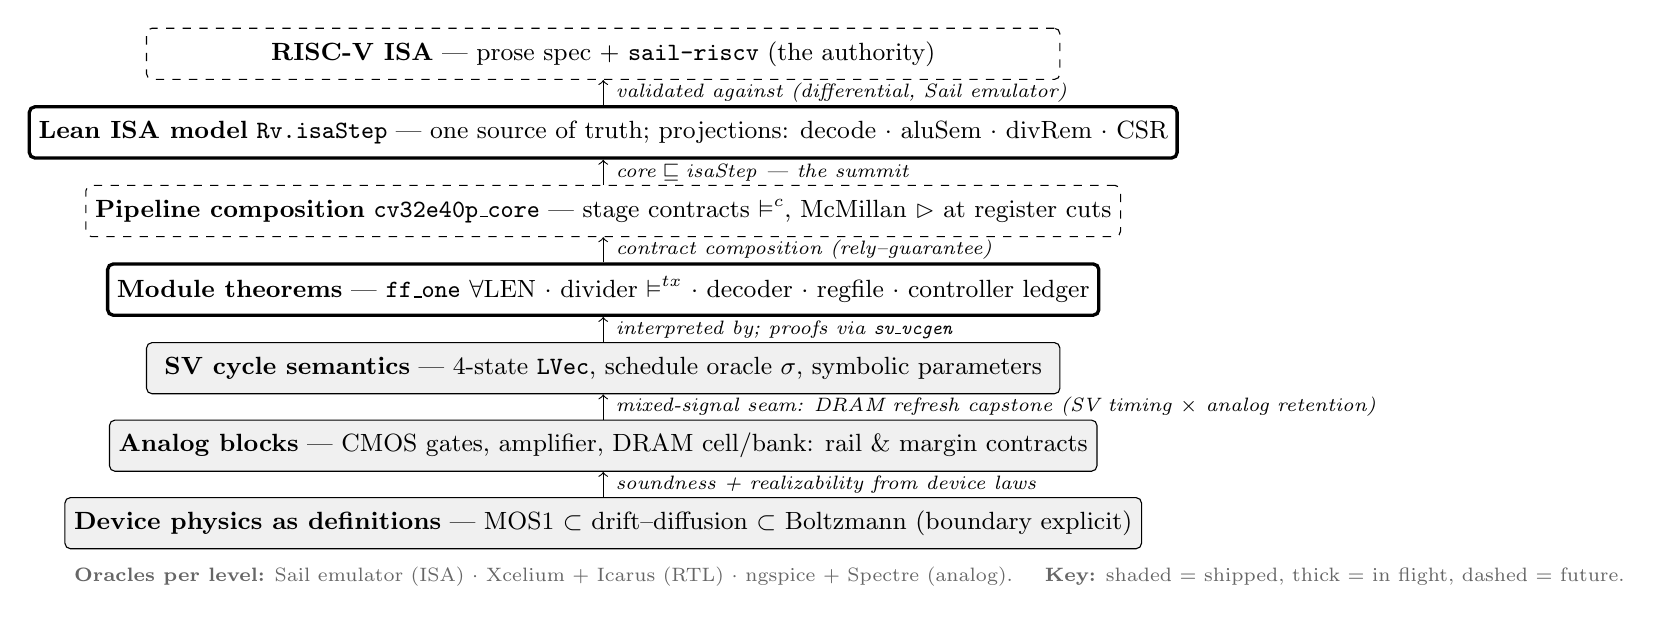
\begin{tikzpicture}[
  lvl/.style={draw, rounded corners=2pt, minimum width=11.6cm, minimum height=6.5mm, align=center, font=\small},
  shipped/.style={lvl, fill=black!6},
  flight/.style={lvl, very thick},
  future/.style={lvl, dashed},
  rel/.style={font=\scriptsize\itshape, midway, right=1pt},
  orc/.style={font=\scriptsize, anchor=west, text=black!60},
  node distance=3.2mm]
\node[future]  (isa)  {\textbf{RISC-V ISA} --- prose spec + \code{sail-riscv} (the authority)};
\node[flight, below=of isa] (model) {\textbf{Lean ISA model} \code{Rv.isaStep} --- one source of truth; projections: decode $\cdot$ aluSem $\cdot$ divRem $\cdot$ CSR};
\node[future, below=of model] (core) {\textbf{Pipeline composition} \code{cv32e40p\_core} --- stage contracts $\vDash^{c}$, McMillan $\rhd$ at register cuts};
\node[flight, below=of core] (mod)  {\textbf{Module theorems} --- \code{ff\_one} $\forall$LEN $\cdot$ divider $\vDash^{tx}$ $\cdot$ decoder $\cdot$ regfile $\cdot$ controller ledger};
\node[shipped, below=of mod] (sem)  {\textbf{SV cycle semantics} --- 4-state \code{LVec}, schedule oracle $\sigma$, symbolic parameters};
\node[shipped, below=of sem] (ana)  {\textbf{Analog blocks} --- CMOS gates, amplifier, DRAM cell/bank: rail \& margin contracts};
\node[shipped, below=of ana] (phys) {\textbf{Device physics as definitions} --- MOS1 $\subset$ drift--diffusion $\subset$ Boltzmann (boundary explicit)};
\draw[->] (model.north) -- (isa.south)  node[rel] {validated against (differential, Sail emulator)};
\draw[->] (core.north)  -- (model.south) node[rel] {$\textit{core} \sqsubseteq \textit{isaStep}$ --- the summit};
\draw[->] (mod.north)   -- (core.south)  node[rel] {contract composition (rely--guarantee)};
\draw[->] (sem.north)   -- (mod.south)   node[rel] {interpreted by; proofs via \code{sv\_vcgen}};
\draw[->] (ana.north)   -- (sem.south)   node[rel] {mixed-signal seam: DRAM refresh capstone (SV timing $\times$ analog retention)};
\draw[->] (phys.north)  -- (ana.south)   node[rel] {soundness + realizability from device laws};
\node[orc] at ([xshift=2mm]isa.east)  {};
\node[orc, anchor=north west] at ([yshift=-1mm]phys.south west) {\textbf{Oracles per level:} Sail emulator (ISA) $\cdot$ Xcelium + Icarus (RTL) $\cdot$ ngspice + Spectre (analog). \quad \textbf{Key:} shaded = shipped, thick = in flight, dashed = future.};
\end{tikzpicture}
\caption{The refinement tower. Every level is a Lean artifact; every arrow is a theorem (or its differential validation); every level has an independent real-world oracle. The digital stack grounds in cycle semantics; the analog stack grounds in device physics with the assurance boundary stated, and the two meet at the DRAM refresh capstone.}
\label{fig:tower}
\end{figure}

\section{The analog half, and where the lanes converge}
Hardware in this project means \emph{both halves}: the digital lanes above
(\code{LeanModels/Sv}, \code{LeanModels/Rv}) and an analog lane that is a first-class
peer, not a satellite. (The \textbf{Python lane}, briefly, is the methodology pathfinder:
\code{py\_vcgen} validated the walker/clause/telescope architecture \code{sv\_vcgen}
transplants, and its real-program benchmark supplies the legibility evidence --- cold
agents with no project context, working from repo docs alone, have proved CPython's
\code{bisect\_left} and real PyPI checksum functions.) The \textbf{analog lane}
(\code{LeanModels/Circuit}, \code{LeanModels/Spice}) parses SPICE decks natively and
treats physics as \emph{definitions}, never axioms: KCL plus device laws \emph{define}
the satisfaction relation, DC operating points are exact over $\mathbb{Q}$ (the harness
prints our exact rational beside ngspice's float --- the simulator approximates
\emph{us}), a restricted MOS transistor tier supports proved CMOS gates, an amplifier
whose gain is a literal \code{deriv} matching ngspice and Spectre to nine digits, and an
8{,}192-cell DRAM bank with kernel-checked deck projection and a cross-coupled sense
amplifier whose metastable state is provably \emph{outside} the correctness theorems.
Three patterns you will recognize crossed over from there: $\forall N$ structural
induction over circuit families predates (and inspired) the SV symbolic-parameters law;
contracts carry \emph{both} inclusions (projection and realization); and the
realizability-pairing rule was born from an audit that found a plausible MOS theorem set
kernel-provably vacuous. The \textbf{endgame} that joins your lane to theirs (Figure~\ref{fig:tower}) is the DRAM
refresh capstone: the SV side proves \emph{``the controller refreshes every row within
$T_{\mathit{ref}}$''} (cycle counting --- \code{sv\_vcgen} territory), the analog side
proves \emph{``a cell retains its bit for at least $T_{\mathit{ref}}$ under a stated
leakage envelope,''} and one composed theorem states \emph{no bit is ever lost} --- a
sentence neither a simulator nor a single-domain tool can even form. Design your module
contracts with that consumer in mind.

\paragraph{Good first contributions.} (a)~Pick one T-select feature (a reduction
operator, part-select) and land it diff-rows-first --- small, complete, teaches the whole
workflow. (b)~Add a lemma to the symbolic-width \code{LVec} pack (append/slice/reduction
algebra) with a \code{\#guard} battery. (c)~When \code{sv\_vcgen} lands, reprove
\code{counter} in clause form --- the regression benchmark needs doing and is the best
tactic tutorial we have. (d)~Draft the FIFO $\forall$\code{DEPTH} proof from gallery
entry~3. (e)~Read the controller contract (gallery entry~10) \emph{skeptically} and file issues
--- fresh eyes on rely clauses are worth more than code. (f)~On the analog side: the
sense amplifier's offset-quantified margin theorem is the documented open residual
(\code{DramDifferentialSenseInitialMargin} is defined but consumed by no theorem) ---
closing it is the analog lane's highest-value open item, and a fine entry point if
device-level work appeals to you.

\section{Where things stand and how we work}
\textbf{Running now}: Phase 2 (Lean ingestion of symbolic envelopes + the
T-select/case-inside/T-reset tier, differential rows first; acceptance: the actual
\code{ff\_one}/\code{popcnt}/divider RTL executing under our interpreter against simulator
traces) and the ISA model build (with Sail-emulator validation). \textbf{Next}: fire
\code{sv\_vcgen} when Phase 2 lands; then the module ladder --- leaves, memory-ish modules,
decoder, FSMs --- then contracts, then the summit. \textbf{House workflow you should adopt}:
gallery-first (statements agreed before machinery); differential rows before semantics;
existing theorem statements are byte-preserved through refactors; every new theorem gets
\code{\#print axioms} pinned (standard axioms only --- no \code{sorry},
\code{native\_decide}, or custom axioms, ever); adversarial audits with kernel-checkable
evidence before landing (they have caught real vacuity twice --- treat them as a gift);
\code{bash tools/ci.sh} is the full local gate and cloud CI mirrors it. \textbf{Reading
order}: this brief; \code{README.md}; \code{docs/sv-design-m0.md} and
\code{docs/sv-spec-surface.md} (lane contract and gallery);
\code{docs/cv32e40p-coverage.md} and \code{docs/cv32e40p-spec-surface.md} (the program);
\code{docs/litreview/SYNTHESIS.md} (why each big design call went the way it did); then
\code{LeanModels/Sv/Semantics.lean} and one example pair
(\code{Examples/system-verilog/counter/}). Welcome aboard --- the summit theorem
($\textit{cv32e40p} \sqsubseteq \textit{isaStep}$, on the shipped core, through our own
front door, at symbolic width) has not been done by anyone; every rung toward it is a
publishable artifact on its own.
\end{document}
